\chapter{Particle Swarm Optimization}\label{cha:pso}
\section{Einleitung}

Hier kommt der Text vom Patrick rein...
Bla

Blubb
\LaTeX
BLABLA

\section{Optimierung von PID Reglern}

In den letzten Jahrzehnten ist das Thema Regelungstechnik oder Prozessregelung
in der Industrie immer wichtiger geworden. Dabei versuchen Regler mechanische
oder elektronische Prozesse zu steuern und Fehler auszugleichen. Ein Beispiel
sei hier ein Elektromotor mit variabler Last. Wenn gefordert wird, dass dieser
mit konstanter Drehzahl l\"auft, muss bei Last\"anderung die angelegte Spannung
ge\"andert werden. Das \"ubernimmt ein Regler. In Grafik
\ref{pic:einfacher_regelkreis} ist ein Standartregelkreis abgebildet. Die
Regelstrecke ist dabei der zu regelnde Elektromotor.

\begin{figure}[hbtp]
    \centering
    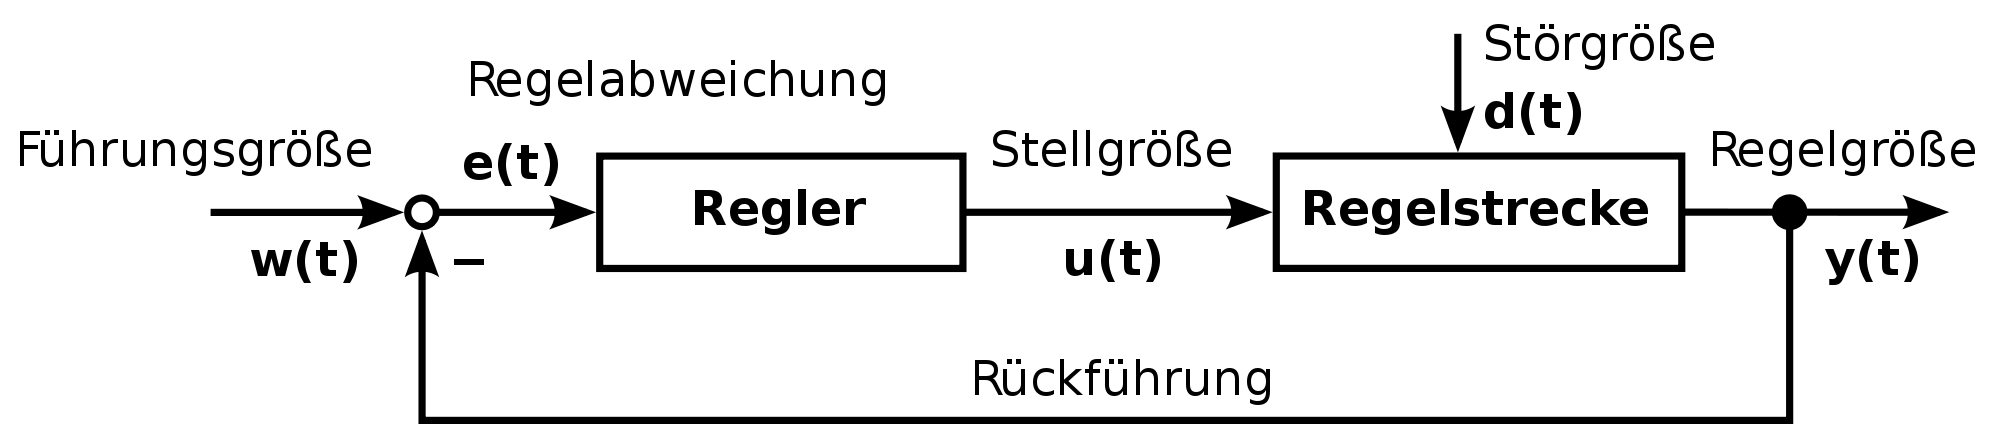
\includegraphics[width=0.8\linewidth]{images/2000px-Einfacher_Regelkreis_n}
    \caption{Standartregelkreis (Quelle: Wikipedia)}
    \label{pic:einfacher_regelkreis}
\end{figure}

Der bekannteste Reglertyp ist der PID-Regler. PID steht dabei f\"ur
\textit{pro\-por\-tional–inte\-gral–deri\-va\-tive}, was auf die drei
Reglerbestandteile bezogen ist. Der Regler besitzt also im Normalfall
proportionale, integrative und differenzielle Anteile. Die Differenzialgleichung
eines PID-Reglers wie folgt gegeben.

\begin{equation}
    u(t)=K_p \left[e(t)+\frac 1{T_i}\int_0^t{e(\tau)}d\tau+\ T_d \frac d{dt}e(t)\right] 
    \label{eq:PID_zeitbereich}
\end{equation}

Dabei ist $K_p$ die Konstante des proportionalen, $T_i$ die des integralen und
$T_d$ dies des differenziellen Anteils. Damit ein Regler Abweichungen schnell
korrigiert ist eine richtige Wahl der genannten Konstanten notwendig.

\subsection{Reglerauslegung}

F\"ur die Wahl der Konstanten des PID-Reglers gibt es verschiedene Methoden. Die
einfachste die Methode von Ziegler und Nichols. Sie ist ein heuristisches
Verfahren, welches auf experimentell ermittelte Werte basiert. Um ein besseres
Regelverhalten zu erzielen sind aber kompliziertere Verfahren notwendig, die
Eigenschaften der Regelstrecke st\"arker einbeziehen. Bekannte Algorithmen sind
\textit{Genetischer Algorithmus} und \textit{Simulierte Abk\"uhlung}
\parencite{bib:pso_pid_gaing}. Da es sich bei den Berechnungen meist um
nichtlineare Optimierungsprobleme handelt, sind sie mit einem sehr hohen
Rechenaufwand verbunden. Der Genetischer Algorithmus (GA) hat dabei noch den
Vorteil dass dieser stark parallelisiert. 

PSO (Kapitel \ref{cha:pso}), als moderner heuristischer Algorithmus zur L\"osung
von nichtlinearen Optimierungsproblemen, bietet sich zur Reglerauslegung an, da
er in kurzer Berechnungszeit schneller konvergierende L\"osungen errechnet.

\subsection{Grundlagen der Reglerauslegung mit PSO}

Um Reglerauslegung mit PSO zu betreiben ist es notwendig, eine f\"ur den
L\"osungsraum g\"ultige Fitnessfunktion zu definieren. Dabei stellt sich die
Frage, was die geforderten Qualit\"atskriterien sind.\\ Ein wichtiges Merkmal
ist die Sollwertabweichung $e(t)=y(t)-w(t)$. \"Uber diese Abweichung sind die
folgenden, oft genutzten Fehlerabweichungen definiert:

\begin{eqnarray}
    IAE&=&\int^{\infty}_0\lvert y(t)-w(t)\rvert dt=\int^{\infty}_0\lvert e(t)\rvert dt \label{eq:IAE} \\
    ISE&=&\int^{\infty}_0 e^2(t) dt \label{eq:ISE} \\
    ITSE&=&\int^{\infty}_0 t\cdot e^2(t) dt \label{eq:ITSE}
\end{eqnarray}

Dabei bedeutet IAE \textit{integrated absolute error} (Integrierter absoluter
Fehler), ISE \textit{ integral of squared-error} (Integrierter quadratischer
Fehler) und ITSE \textit{integrated of time-weighted-squared-error}
(integrierter zeitlich-gewichteter quadratischer Fehler).

In einer Studie \parencite{bib:pso_pid_gaing} wurde eine alternative
Fitnessfunktion benutzt.

\begin{equation}
    W(K)=(1-e^{-\beta})\cdot (M_p+E_{ss})+e^{-\beta}\cdot (t_s-t_r) \label{eq:fit_gaing}
\end{equation}

Die Fitnessfunktion $W(K)$ (Gleichung \ref{eq:fit_gaing}) bezieht dabei folgende
Qualit\"atskriterien (anschaulich in Grafik \ref{img:stepresponse}) ein. Mit der
Konstanten $\beta$ dabei zus\"atzliche Eigenschaften beeinflusst werden. Ein
Wert von $\beta$ gr\"o\ss er als 0,7 reduziert dabei die \"Uberschwingweite und
die Sollwertabweichung. Ein $\beta$ kleiner als 0,7 reduziert die Anstiegszeit
und die Einschwingdauer.

\begin{eqnarray}
    \textrm{Sollwertabweichung}\quad E_{ss}&=&\lim_{t \to \infty}e(t)\\
    \textrm{peak time (Zeit zum ersten Maximum)} &=& t_p\\
    \textrm{Verz\"ogerungszeit (Zeit, bis 50\% erreicht sind)} &=& t_d \\
    \textrm{Anstiegszeit (Zeit, bis 100\% erreicht sind)} &=& t_r \\
    \textrm{maximale \"Uberschwingweite} &=& M_p 
\end{eqnarray}

\begin{figure}[hbtp]
    \centering
    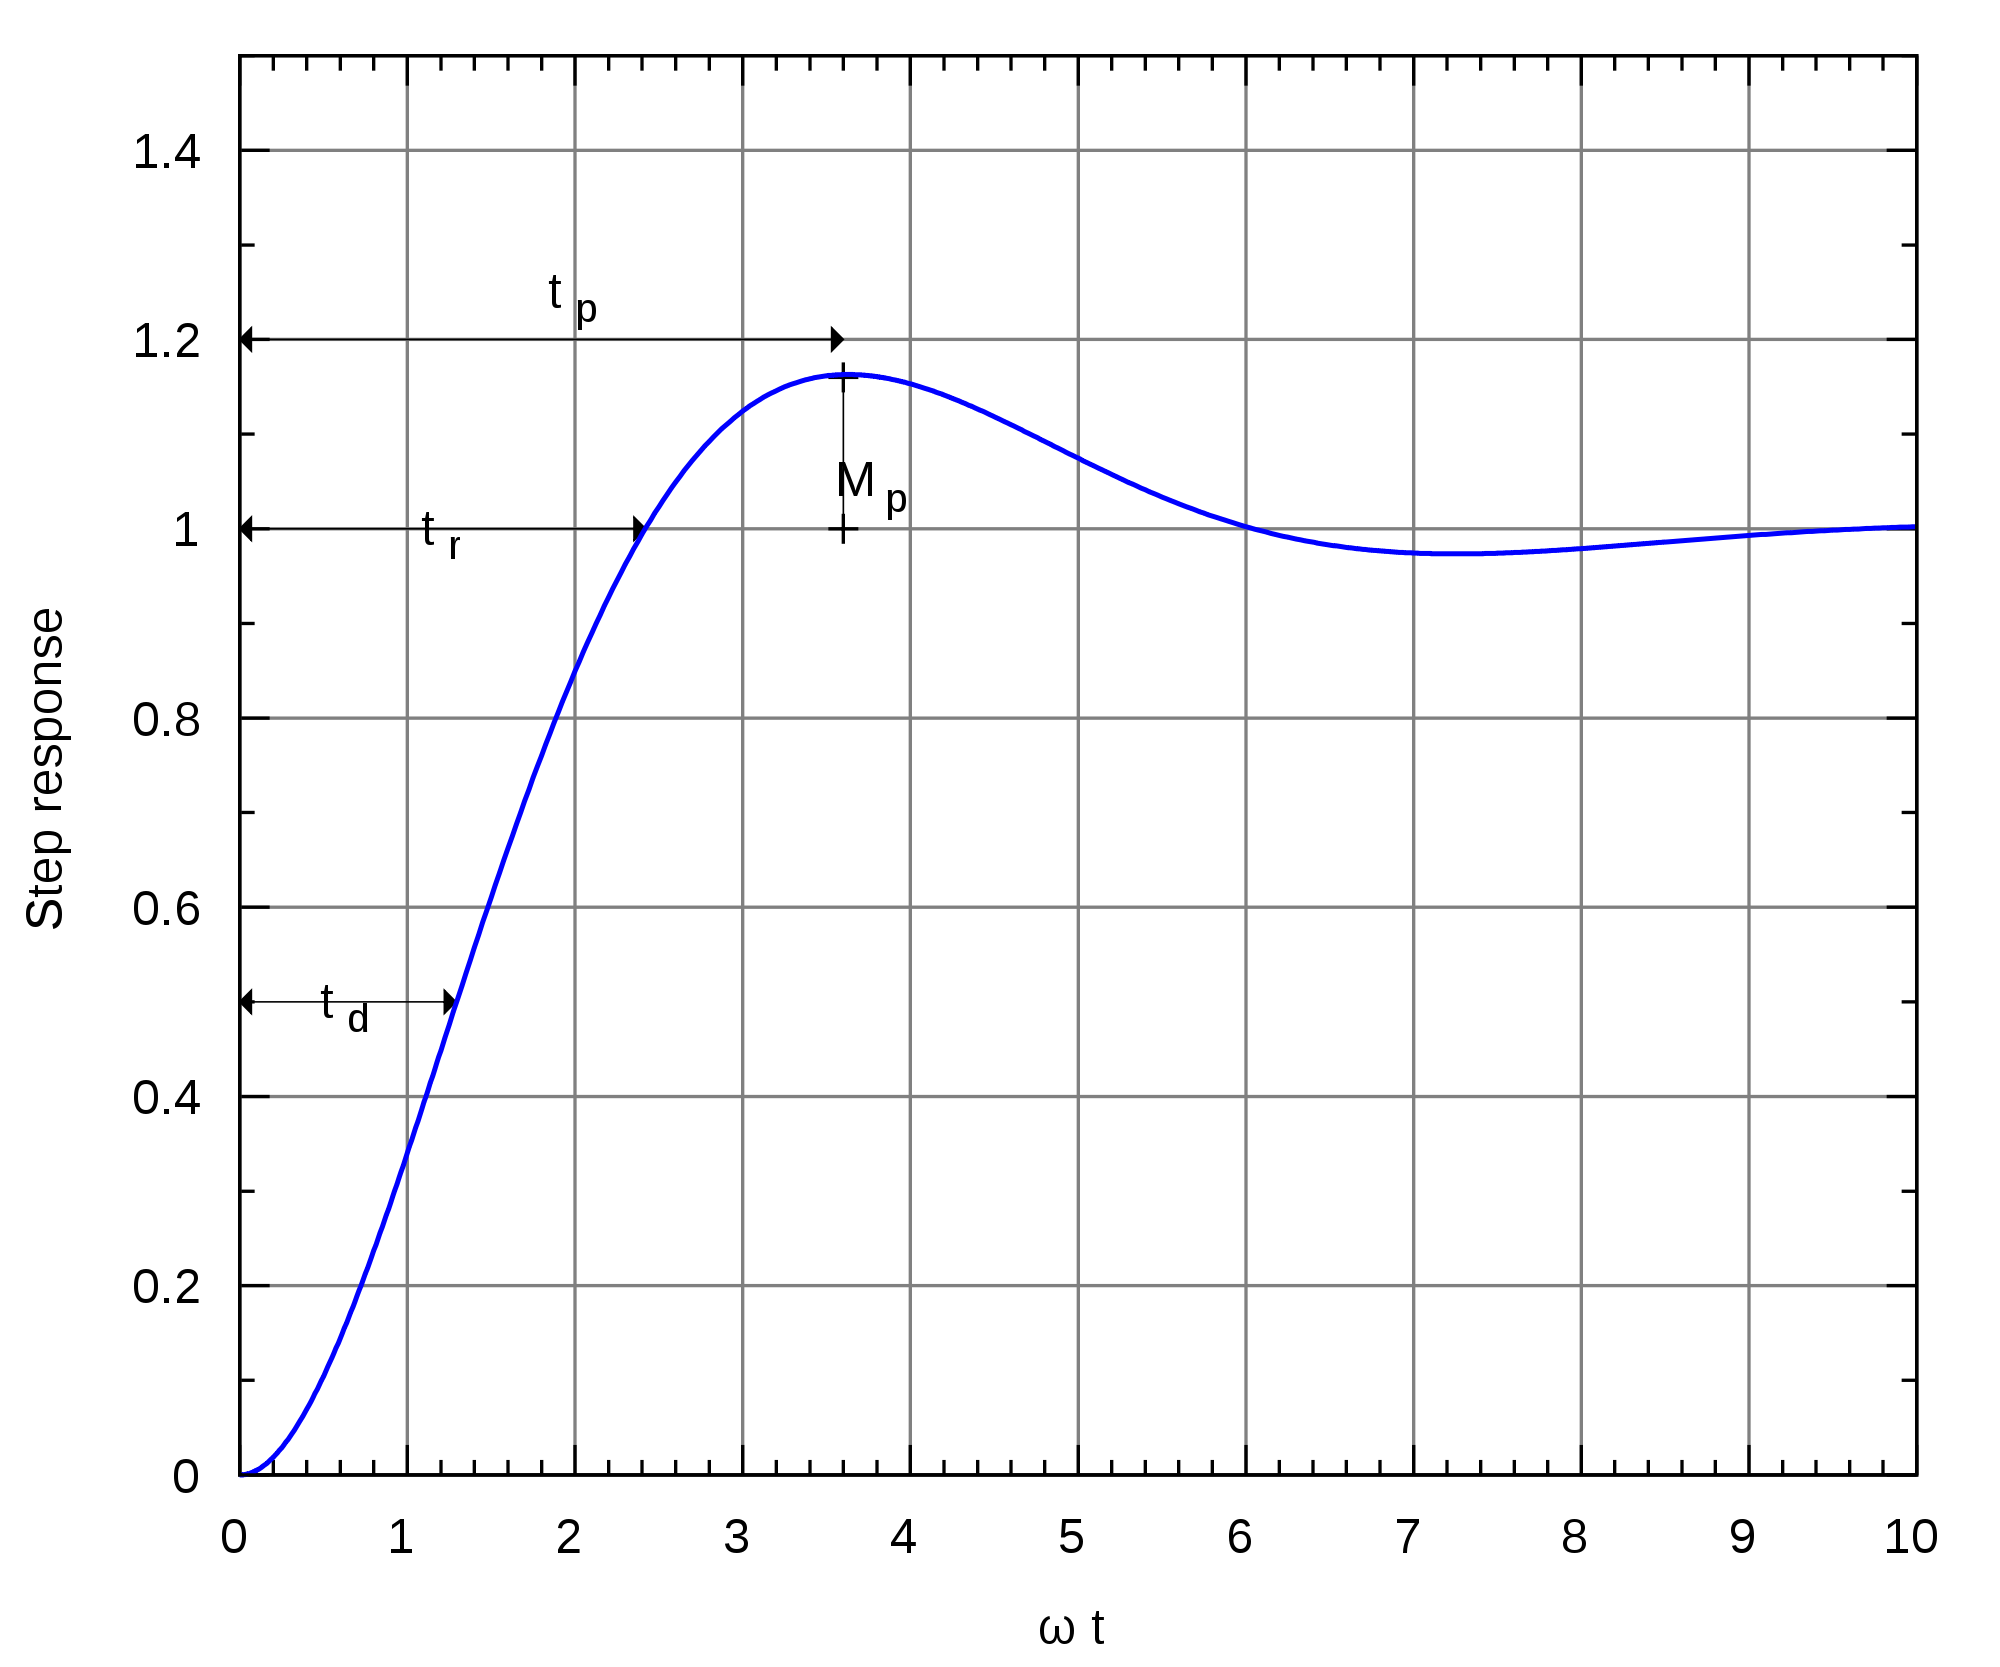
\includegraphics[width=0.8\linewidth]{images/2000px-Second_order_under-damped_response}
    \caption{Sprungantwort\protect\footnotemark eines Systems (Quelle: Wikipedia)}
    \label{img:stepresponse}
\end{figure}

\footnotetext{Reaktion eines Systems auf die Sprungfunktion der H\"ohe eins} Ein
gro\ss er Vorteil der von Gaing benutzten Fitnessfunktion ist, dass sie im
Gegensatz zu \eqref{eq:IAE}-\eqref{eq:ITSE} mehrere Qualit\"atsparameter
ber\"ucksichtigt.

Ein wichtiges Qualit\"atsmerkmal eines Reglers, bzw. des Regelkreises ist deren
Stabilit\"at. Die Stabilit\"at beschreibt die Reaktion des Regelkreises auf
beschr\"ankte Eingangssignale. Gefordert wird normalerweise BIBO-Stabilit\"at
(Bounded Input Bounded Output). Das bedeutet, dass ein System auf ein
beliebiges, aber beschr\"anktes Eingangssignal mit einem beschr\"ankten
Ausgangssignal antwortet. Mathematisch ausgedr\"uckt:

\begin{equation}
    |y(t)| \leq C \cdot M < \infty\qquad\forall|w(t)| \leq M\qquad C,M\in \mathbb{R}
\end{equation}

Stabilit\"at kann zum Beispiel mit dem Hurwitz-Kriterium oder dem Routh–Hurwitz Kriterium \"uberpr\"uft werden \parencite{routh1877treatise}.

\subsection{Reglerauslegung mit PSO nach Gaing}

Die Berechnung der Reglerparameter erfolgt f\"ur einen PID-Regler im Laplace-Bereich. Durch Laplace-Transformation von Gleichung \eqref{eq:PID_zeitbereich}.

\begin{equation}
    \mathcal{L}\left\{u\right\}(s) =\int_{0}^{\infty} \mathrm{e}^{-st} u(t)\,\mathrm{d}t=k_p+\frac{k_i}{s}+k_ds \qquad s\in\mathbb{C}.
\end{equation}

Auch wird anstatt der Fitnessfunktion $W(K)$ ihr Kehrwert $f=1/W(K)$ zur Berechnung benutzt.
In der Studie von Gaing \parencite{bib:pso_pid_gaing} wurde der Reglerparametervektor $K=[k_p,k_i,k_d]$ wie folgt in neun Schritten ermittelt.

\underline{\textbf{AB HIER M\"USSEN REFERENZEN ZUM PSO KAPITEL EINGEARBEITET WERDEN}}\\
--> ROHVERSION, INDIVIDUUM vs PARTIKEL

\begin{enumerate}
    \item Definieren der Ober- und Untergrenzen der drei Reglerparameter $k_i$, also das Festlegen des L\"osungsraumes. Zuf\"alliges initialisieren der Parameter der Testpopulation wie Position, Geschwindigkeit, pbest und gbest.
    \item Individuelles \"uberpr\"ufen der Stabilit\"at jedes $K$ der Population und jeweils berechnen der Optimierungsparameter $E_{ss}$, $M_p$, $t_r$ und $t_s$.
    \item Auswerten der Fitnessfunktion $f$ f\"ur jedes Individuum
    \item Vergleichen aller Werte pbest und ggf. ermitteln eines neues gbest.
    \item Zuf\"alliges Ver\"andern der Geschwindigkeit jedes Individuums
        \begin{eqnarray}
            v_{j,g}^{(t+1)}&=&w\cdot v_j^{(t)}+c_1\cdot rand() [pbest_{j,g}-k^{(t)}_{j,g}]+c_2\cdot rand() [gbest{g}-k^{(t)}_{j,g}] \nonumber\\
            j&=&1,2...n\nonumber\\
            g&=&1,2,3\nonumber
        \end{eqnarray}
        wobei f\"ur $g=1$ $v_{j,1}$ die \"Anderung der Geschwindigkeit von $k_p$ oder f\"ur $g=2$ $v_{j,2}$ die \"Anderung der Geschwindigkeit von $k_i$ repr\"asentiert.
    \item Wenn $v_{j,g}^{(t+1)}>V_g^{max}$, dann $v_{j,g}^{(t+1)}=V_g^{max}$ und wenn $v_{j,g}^{(t+1)}<V_g^{min}$, dann $v_{j,g}^{(t+1)}=V_g^{min}$
    \item \"Anderung der Position aller K Werte wie folgt
        \begin{equation}
            k^{(t+1)}_{j,g}=k^{(t)}_{j,g}+v_{j,g}^{(t+1)}\quad \textrm{mit}\quad k^{min}_{g} \leq k^{(t+1)}_{j,g} \leq k^{max}_{g}
        \end{equation}
        wobei $k^{min}_{g}$ und $k^{max}_{g}$ die Ober- und Untergrenzen des Jeweiligen Reglerparameters bezeichnen.
    \item Wenn die maximale Anzahl an Iteration erreicht ist weiter mit 9., sonst gehe zu Schritt 2.
    \item Das Individuum, welches das letzte gbest generiert hat enth\"alt die optimalen Reglerparameter.
\end{enumerate}

Gaing konnte in seiner Studie zeigen, dass die mit PSO Methode gefundenen Reglerparameter ein sehr gutes Verhalten zeigten. Dabei wurde der Algorithmus an dem in Grafik \ref{img:avr_sys} gezeigten System getestet.

\begin{figure}[hbtp]
    \centering
    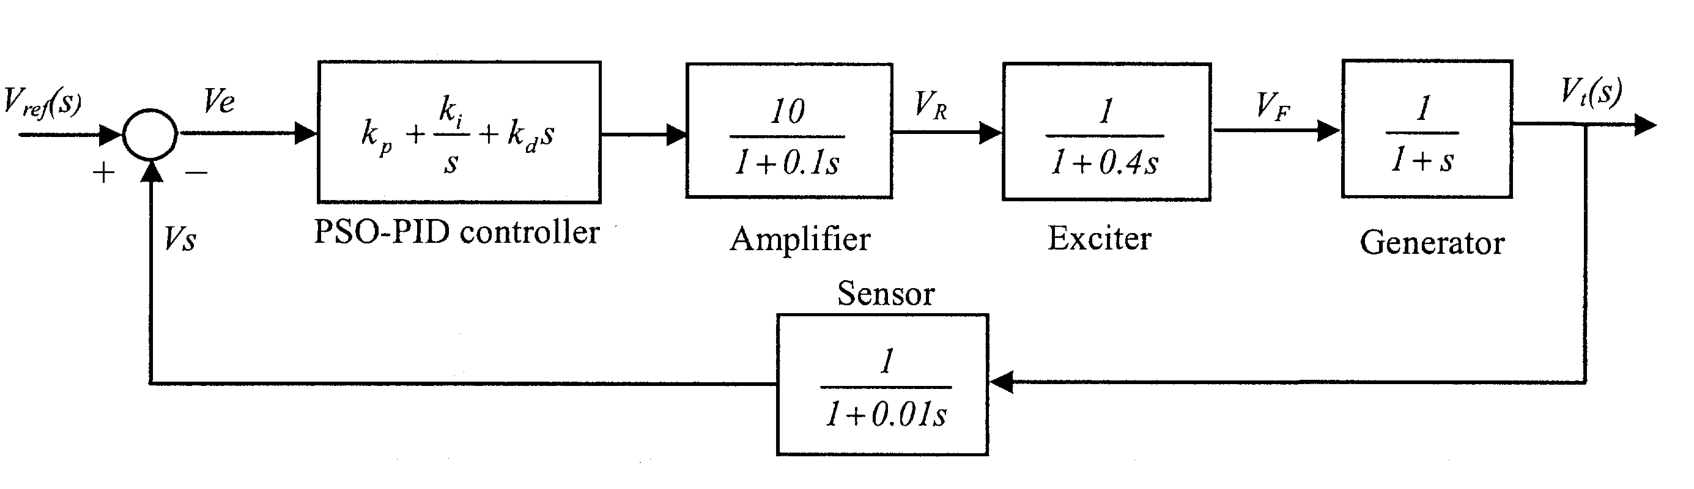
\includegraphics[width=0.8\linewidth]{images/avr_system}
    \caption{Blockdiagramm des AVR Systems mit PID Regler}
    \label{img:avr_sys}
\end{figure}

In Grafik \ref{img:avr_ohne_regler} ist die Sprungantwort des Systems ohne Regelung zu sehen. Das System strebt zwar gegen einen Endwert, schwingt dabei aber sehr stak und die Sollwertabweichung ist auch gr\"o\ss er Null.
\begin{figure}[hbtp]
    \centering
    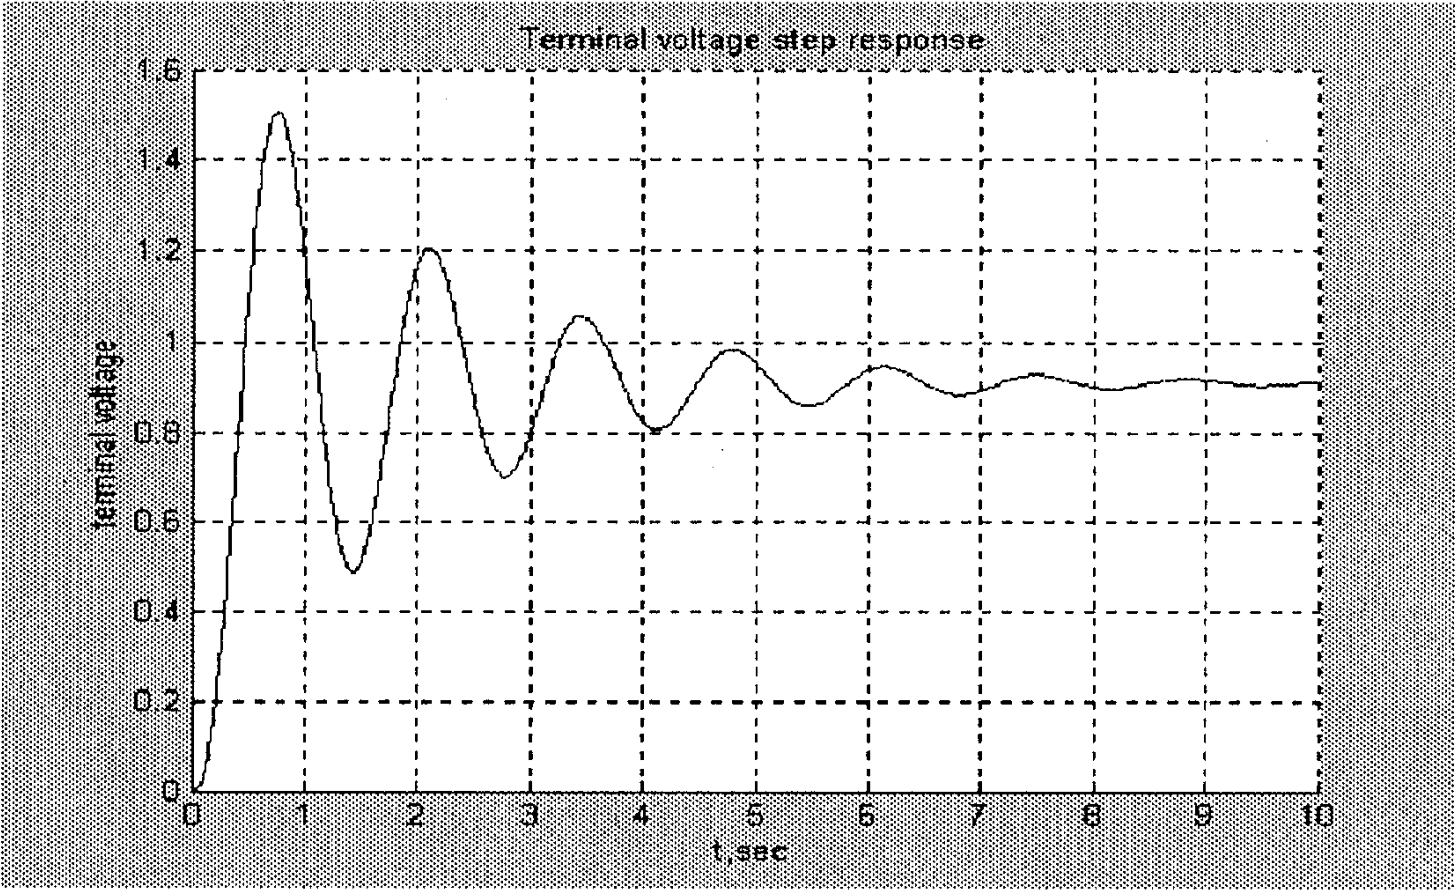
\includegraphics[width=0.8\linewidth]{images/avr_ohne_regler}
    \caption{Sprungantwort des AVR Systems ohne Regler}
    \label{img:avr_ohne_regler}
\end{figure}

In Grafik \ref{img:avr_mit_regler} sind die Sprungantworten des geregelten
Systems durch PID-Regler mit PSO-Parametern und PID-Regler mit Parametern des
Genetischen Algorithmus. Gerechnet wurde dabei mit $\beta = 1,0$ und $n=50$
Individuen. Beide Algorithmen kommen auf eine Sollwertabweichung von
$e(\infty)=0$, besitzen aber unterschiedliche \"Uberschwingweiten und
Anstiegszeiten. In den Versuchen von Gaing erreichte der GA eine etwas k\"urzere
Berechnungszeit als der PSO Algorithmus. Dies k\"onnen die errechneten Werte des
PSO Algorithmus durch eine bessere Sollwertfolge und eine geringere
\"Uberschwingweite ausgleichen.

Abschlie\ss end kann man sagen, dass beide Berechnungsverfahren ihre
Berechtigung haben, der PSO Algorithmus liefert aber auf \"Uberschwingweite
bezogen wesentlich bessere Ergebnisse.

\begin{figure}[hbtp]
    \centering
    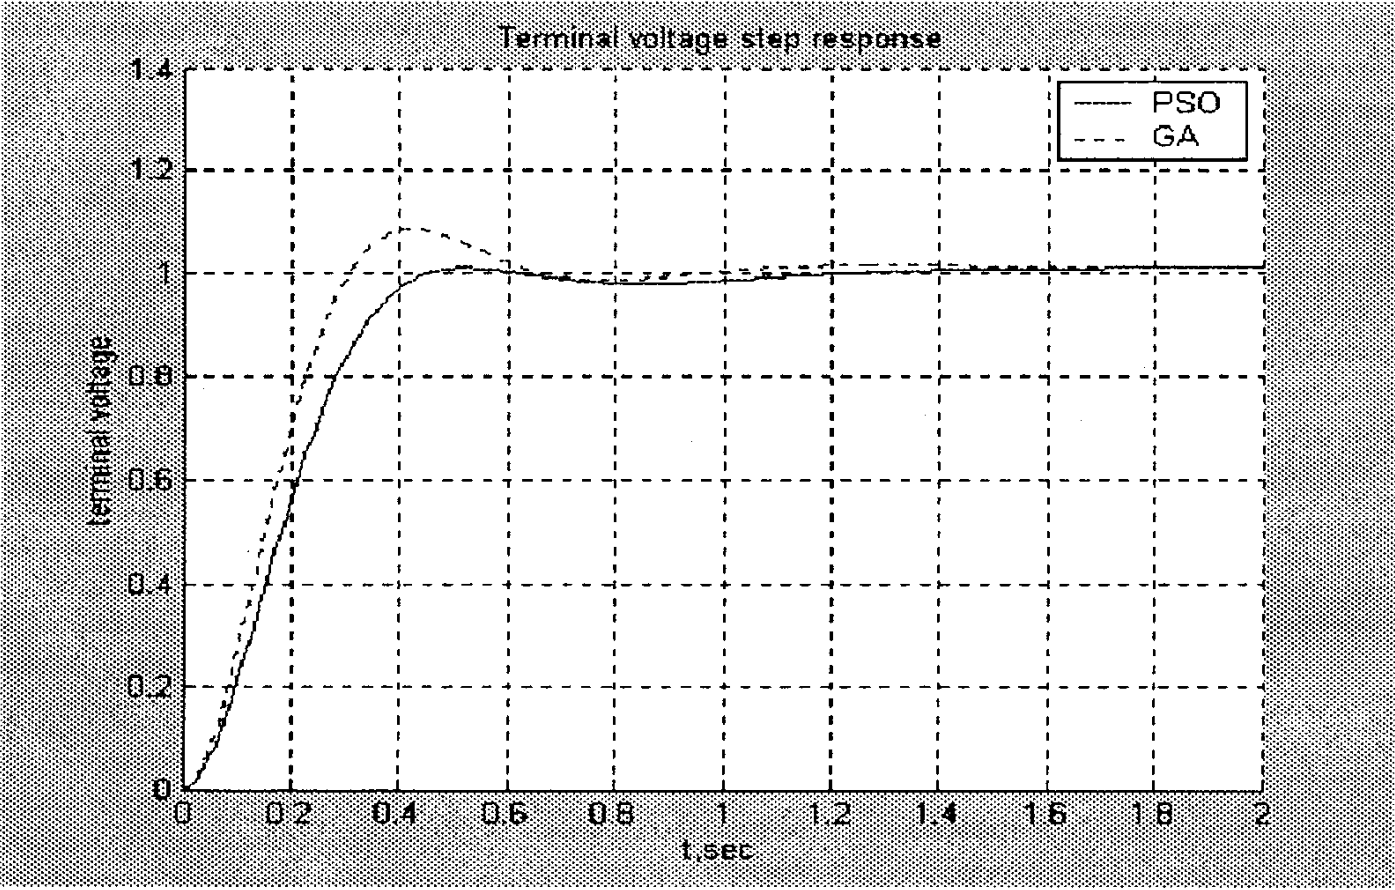
\includegraphics[width=0.8\linewidth]{images/avr_mit_regler}
    \caption{Sprungantwort des PID-geregelten AVR Systems mit PSO und GA Parametern}
    \label{img:avr_mit_regler}
\end{figure}
